\chapter{A respiração}\label{ch:g4:breathing}

Prenda a \omterm{def:g4:breathing:movements}{respiração} e comece a contar. Bem antes de um minuto, o seu
peito exige, cada vez com mais urgência, se mexer de novo. Você pode
pular uma refeição, o \omterm{prop:g1:healthy-habits:needs}{sono} pode esperar até a noite --- mas o ar é
necessário \emph{agora}, o tempo todo, umas quinze vezes por minuto.
O que é tão urgente numa golfada de ar?

\section{Os movimentos respiratórios}

\begin{definition}[Inspirar e expirar]\label{def:g4:breathing:movements}
\emph{Respirar}\index{respiração} é a alternância sem fim de dois
movimentos:
\begin{itemize}
  \item \emph{inspirar} (a inspiração)\index{inspiração}: o peito
        se expande e o ar entra pelo nariz ou pela boca;
  \item \emph{expirar} (a expiração)\index{expiração}: o peito
        relaxa e o ar volta para fora.
\end{itemize}
Em repouso, o par se repete umas $15$ vezes por minuto --- mais
rápido nos bebês, mais rápido no esforço --- sem que você precise
pensar nisso.
\end{definition}

\begin{example}[Observando os movimentos]\label{ex:g4:breathing:watch}
Mãos espalmadas nas \omterm{def:g3:bones-and-muscles:skeleton}{costelas}: ao inspirar, a caixa torácica sobe e
alarga debaixo das suas palmas; ao expirar, ela afunda de novo. O
flanco de um gato dormindo mostra a mesma subida e descida. Os
movimentos nunca param --- acordado, dormindo, do primeiro choro ao
último dia.
\end{example}

\section{Para onde vai o ar}

\begin{definition}[Os órgãos da respiração]\label{def:g4:breathing:organs}
O ar inspirado passa pelo nariz (ou pela boca) e desce pela
\emph{traqueia}\index{traqueia} --- o tubo firme e cheio de anéis que
você sente na frente do pescoço ---, que se divide em dois ramos, um
para cada \emph{pulmão}\index{pulmão}. Os pulmões, dois órgãos
esponjosos que enchem a caixa torácica (atrás das \omterm{def:g3:bones-and-muscles:skeleton}{costelas} da
\cref{def:g3:bones-and-muscles:skeleton}), terminam em milhões de
bolsinhas de ar, cada uma envolvida por vasos sanguíneos finíssimos.
\end{definition}

\begin{omfigure}
\begin{tikzpicture}
  \node[anchor=south west, inner sep=0] (img) at (0,0)
    {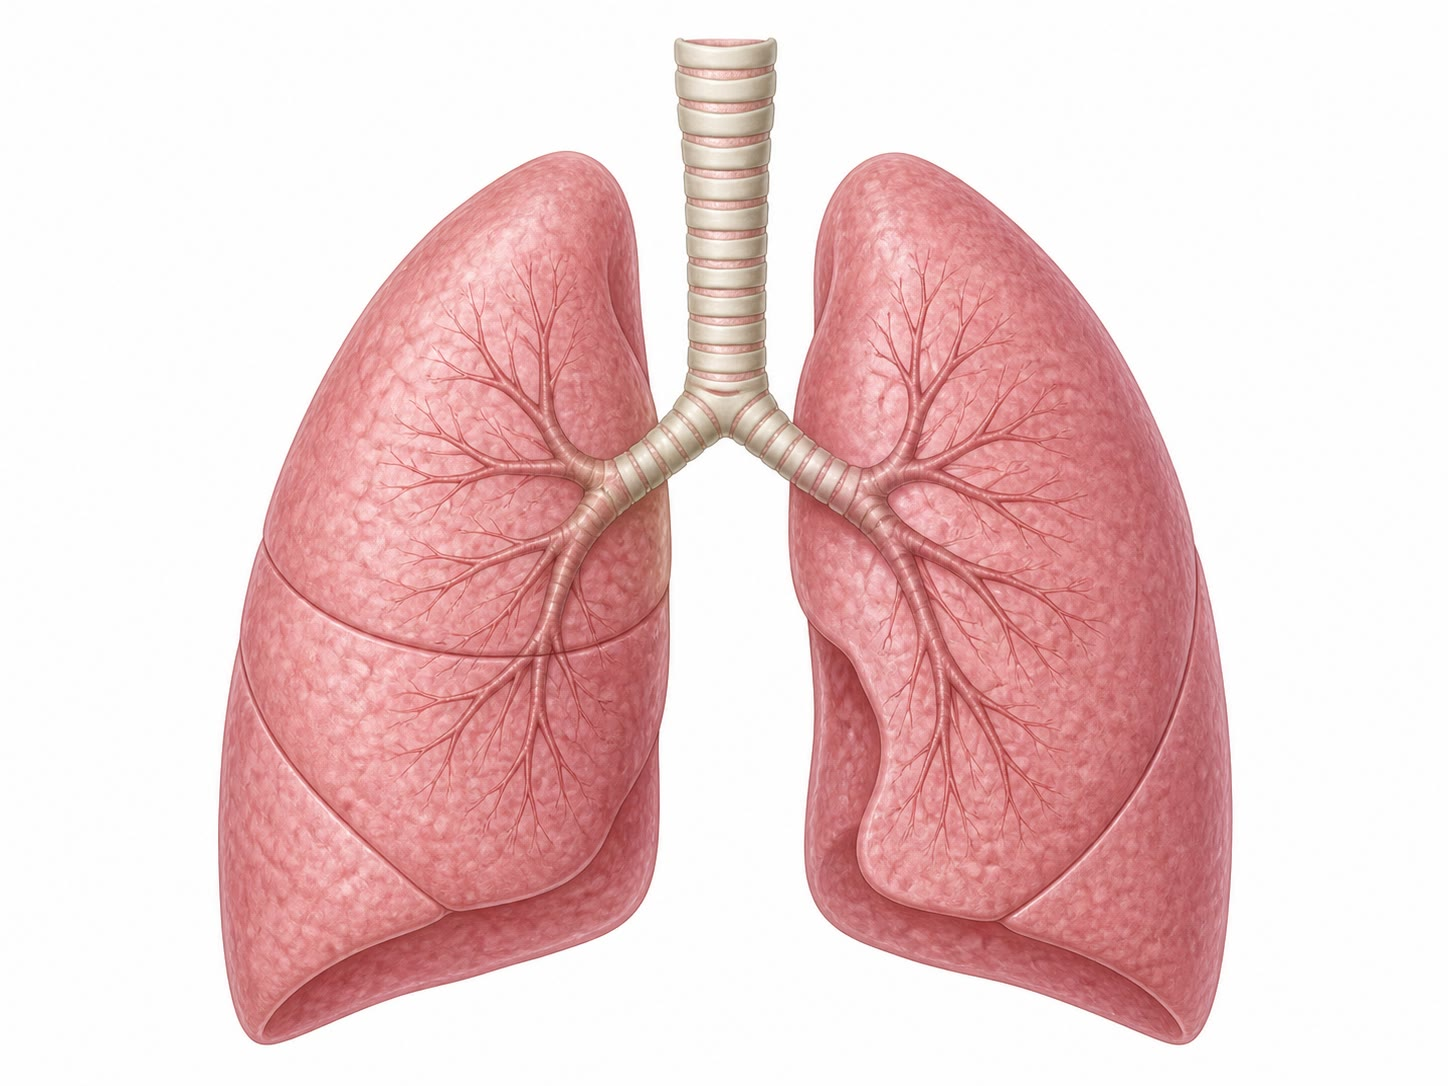
\includegraphics[width=0.58\linewidth]{images/book1/ai/fig-lungs.jpg}};
  \begin{scope}[x={(img.south east)}, y={(img.north west)},
      every node/.style={font=\small}]
    \draw[omDef, thick] (0.53,0.88) -- (0.74,0.93) node[right] {traqueia};
    \draw[omDef, thick] (0.585,0.61) -- (1.03,0.64)
      node[right, align=left] {os dois\\ ramos};
    \draw[omDef, thick] (0.28,0.28) -- (0.11,0.13)
      node[below] {pulmão};
  \end{scope}
\end{tikzpicture}

{\small O caminho de uma golfada de ar: \omterm{def:g4:breathing:organs}{traqueia}, dois ramos, dois
pulmões --- e, nas pontas mais finas dos ramos, milhões de bolsinhas
de ar envolvidas por vasos sanguíneos finíssimos, pequenas demais
para aparecer nesta escala.}
\end{omfigure}

\begin{remark}[Esponjoso de propósito]\label{rem:g4:breathing:sponge}
Milhões de bolsinhas em vez de dois sacos simples: é de novo o
truque do \omterm{def:g4:journey-of-food:tract}{intestino delgado}
(\cref{rem:g4:journey-of-food:surface}). Todas essas paredes de
bolsinha somam uma superfície enorme de encontro entre o ar e o
\omterm{prop:g4:journey-of-food:absorb}{sangue} --- do tamanho de meia quadra de tênis, dobrada dentro do seu
peito.
\end{remark}

\section{Para que serve a respiração}

\begin{proposition}[Pegar oxigênio, devolver gás carbônico]\label{prop:g4:breathing:exchange}
O ar é uma mistura de gases, e o corpo quer um deles: o
\emph{oxigênio}\index{oxigênio}. Nas bolsinhas dos pulmões, o
oxigênio do ar fresco passa para o \omterm{prop:g4:journey-of-food:absorb}{sangue}, que o entrega a todas as
partes do corpo; ali ele é usado, junto com os \omterm{def:g4:journey-of-food:digestion}{nutrientes}, para
liberar a \omterm{prop:g3:balanced-diet:jobs}{energia} da \cref{prop:g3:balanced-diet:jobs}. O gás
residual do corpo, o \emph{gás carbônico}\index{gás carbônico}, faz
a viagem de volta e é expirado. O ar expirado tem menos oxigênio e
mais gás carbônico que o ar inspirado --- e essa diferença é
justamente \emph{para} o que a \omterm{def:g4:breathing:movements}{respiração} serve.
\end{proposition}
\admitted

\begin{example}[Por que correr tira o fôlego]\label{ex:g4:breathing:running}
Numa corrida, as suas \omterm{def:g1:my-body:parts}{pernas} queimam \omterm{prop:g3:balanced-diet:jobs}{energia} depressa --- então
precisam de oxigênio depressa. A \omterm{def:g4:breathing:movements}{respiração} atende: de umas $15$
respirações calmas por minuto para $40$ ou mais, e bem fundas,
enquanto o coração (o \cref{ch:g4:heart-and-blood} conta o lado
dele) dispara para acelerar as entregas. A ofegada depois da corrida
é o corpo acertando as contas de oxigênio.
\end{example}

\begin{example}[O espelho embaçado]\label{ex:g4:breathing:mirror}
Assopre num espelho frio: névoa. O ar expirado volta mudado ---
aquecido, umedecido e, sem aparecer, mais pobre em oxigênio e mais
rico em gás carbônico. O espelho mostra a umidade; a troca de gases,
que ele não consegue mostrar, é a parte importante.
\end{example}

\begin{omfigure}
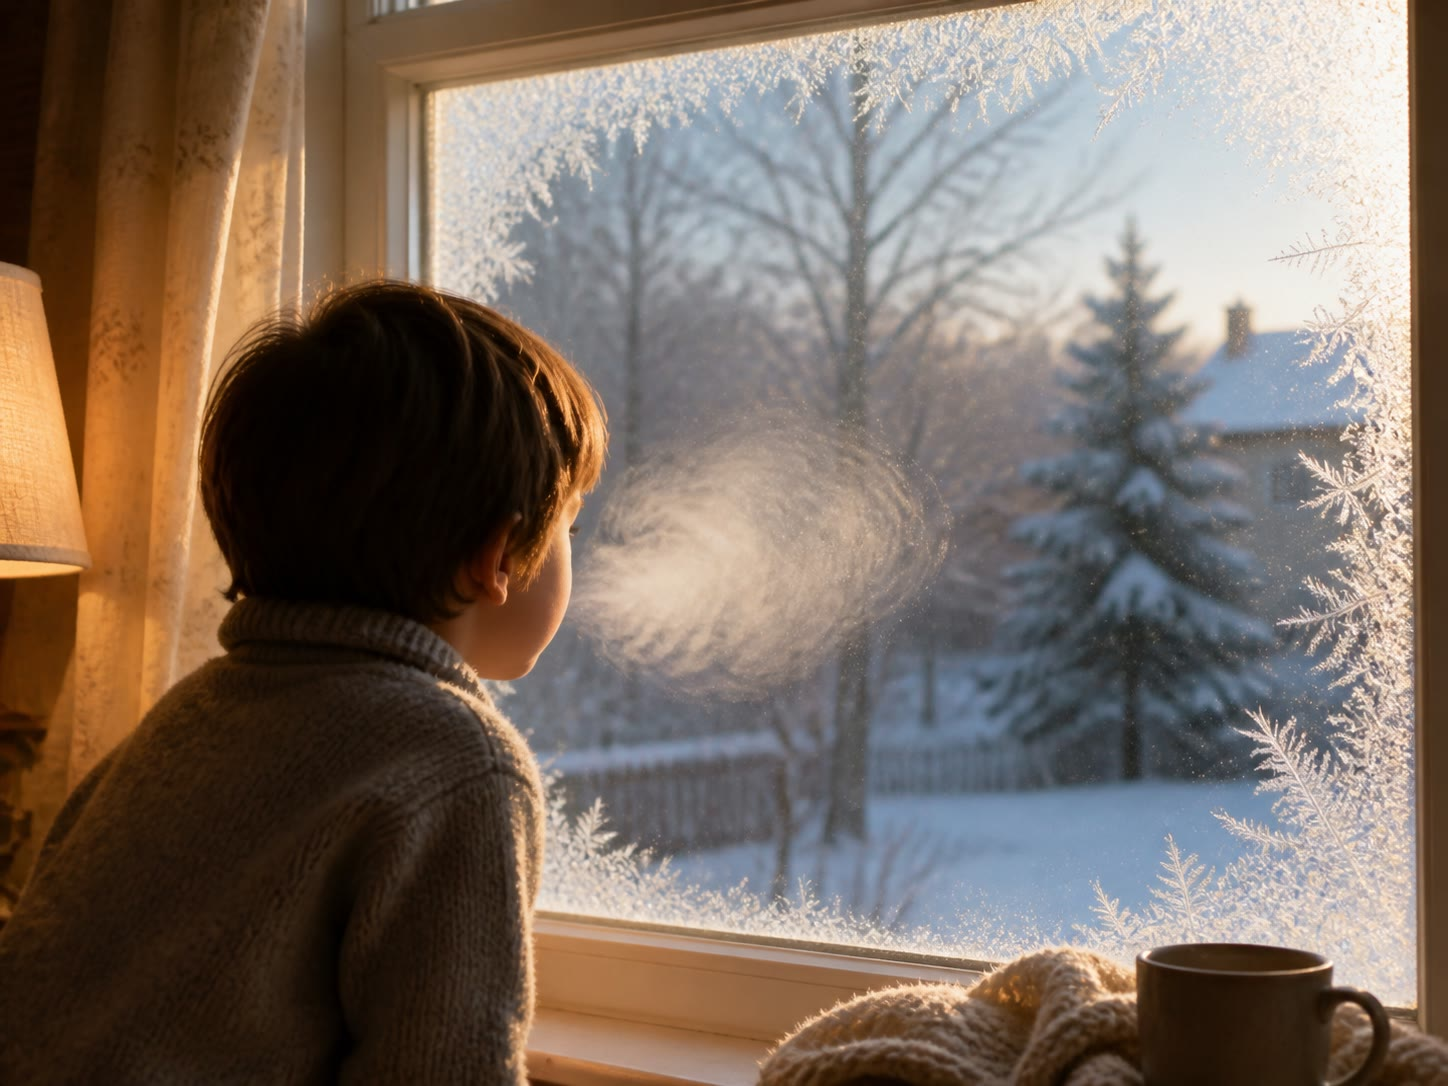
\includegraphics[width=0.56\linewidth]{images/book1/ai/g4-breathing-mist.jpg}

{\small O ar expirado tornado visível: quente, úmido --- e, sem
aparecer, mais pobre em oxigênio e mais rico em gás carbônico.}
\end{omfigure}

\begin{method}[Cuidar da respiração]\label{met:g4:breathing:care}
\begin{enumerate}
  \item Areje os cômodos todo dia --- muita gente respirando num
        cômodo fechado deixa o ar viciado e rico em gás carbônico;
  \item respire pelo nariz no ar frio ou empoeirado: ele aquece,
        umedece e filtra;
  \item corra, nade, brinque --- pulmões e \omterm{def:g3:bones-and-muscles:muscle}{músculos} respiratórios
        exercitados ficam mais fortes e mais profundos;
  \item mantenha a fumaça longe dos seus pulmões: ela suja as
        bolsinhas delicadas, e elas só se limpam devagar.
\end{enumerate}
\end{method}

\section{Exercícios}

\begin{exercise}[$\star$]\label{exo:g4:breathing:1}
Diga os dois movimentos respiratórios e o que o peito faz em cada
um.
\end{exercise}

\begin{exercise}[$\star$]\label{exo:g4:breathing:2}
Trace o caminho de uma golfada de ar, do nariz até as bolsinhas de ar.
\end{exercise}

\begin{exercise}[$\star$]\label{exo:g4:breathing:3}
Mais ou menos quantas vezes por minuto respira uma criança em
repouso e tranquila? O que acontece com esse número durante uma
corrida, e por quê?
\end{exercise}

\begin{exercise}[$\star$]\label{exo:g4:breathing:4}
Que gás o corpo pega do ar, e qual ele devolve? Onde exatamente
acontece a troca?
\end{exercise}

\begin{exercise}[$\star$]\label{exo:g4:breathing:5}
Em que o ar expirado difere do ar inspirado? Diga três diferenças.
\end{exercise}

\begin{exercise}[$\star$]\label{exo:g4:breathing:6}
Por que os pulmões são construídos como milhões de bolsinhas em vez
de dois sacos simples? Que outro órgão deste ano usa o mesmo truque?
\end{exercise}

\begin{exercise}[$\star$]\label{exo:g4:breathing:7}
Por que é melhor respirar pelo nariz num dia gelado ou empoeirado?
\end{exercise}

\begin{exercise}[$\star$]\label{exo:g4:breathing:8}
Faça a experiência: sentado com calma, conte as suas respirações
durante um minuto. Depois faça vinte polichinelos e conte de novo.
Informe os dois números e explique a mudança.
\end{exercise}

\begin{exercise}[$\star\star$]\label{exo:g4:breathing:9}
As refeições podem esperar horas; a \omterm{def:g4:breathing:movements}{respiração} não espera um minuto.
O que isso diz sobre quanto oxigênio o corpo guarda de reserva,
comparado com as \omterm{def:g3:animals-through-seasons:active}{reservas de alimento} dele?
\end{exercise}

\begin{exercise}[$\star\star$]\label{exo:g4:breathing:10}
Uma sala de aula fica ``abafada'' no fim da manhã. O que mudou no ar
dela, segundo a \cref{prop:g4:breathing:exchange}, e o que o
\cref{met:g4:breathing:care} receita?
\end{exercise}

\begin{exercise}[$\star\star\star$]\label{exo:g4:breathing:11}
A truta não tem pulmões: a água passa pelas brânquias emplumadas
dela, e o oxigênio \emph{dissolvido na água} passa ali para o \omterm{prop:g4:journey-of-food:absorb}{sangue}
dela. Que trabalho as brânquias e os pulmões dividem? E por que uma
truta sufoca no ar, onde o oxigênio é abundante? (Dica: fora da
água, as superfícies emplumadas das brânquias desabam e grudam umas
nas outras.)
\end{exercise}
